\documentclass{article}

% Required packages for Tikz diagrams
\usepackage{pgf, tikz, amsmath, amsfonts}     
     \usetikzlibrary{external}
     \tikzexternalize % activate!
\usetikzlibrary{arrows, automata, positioning}

\begin{document}

%  \begin{tikzpicture}[
%      > = stealth,                 % arrow head style
%      shorten > = 1pt,             % don't touch arrow head to node
%      auto, node distance = 1.3cm, % distance between nodes
%      semithick                    % thicker arrows
%    ]
%    
%    \tikzstyle{S1}=[      % Defines style for Square 
%      fill = black!15,    % Black with transparency 15%
%      minimum size = 8mm  
%    ]
%    
%    \tikzstyle{R1}=[      % Defines style for Round 
%      circle,             % Changes shape
%      fill = black!15,
%      minimum size = 8mm
%    ]
%    
%    % DO NOT FORGET ; AT THE END OF EACH SENTENCE!!!
%    
%    % Definition of the nodes
%    % \node[style] (name) [relative_position] {Text};
%    % Relative positions: left, right, above, below, above left, etc.
%    \node[S1] (y) {$y_{i}$};
%    \node[R1] (theta) [above of=y] {$\theta_{i}$};
%    \node[S1] (n) [right of=theta] {$n_i$};
%    \node[R1] (beta1) [above of=theta] {$\beta_1$};
%    \node[R1] (beta0) [left of=beta1] {$\beta_0$};
%    \node[S1] (x) [right of=beta1] {$x_i$};
%
%    % Definition of the edges
%    \path[->] (theta) edge node {} (y);
%    \path[->] (n) edge node {} (y);
%    \path[->,dashed] (beta0) edge node {} (theta);
%    \path[->,dashed] (beta1) edge node {} (theta);
%    \path[->,dashed] (x) edge node {} (theta);
%
%  \end{tikzpicture}
  
  
  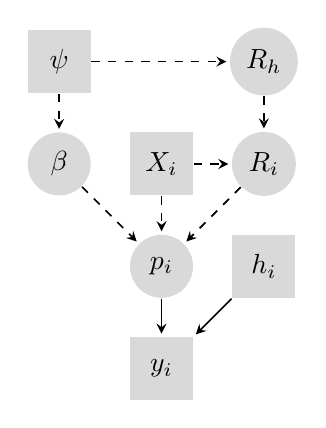
\begin{tikzpicture}[
  > = stealth,                 % arrow head style
  shorten > = 1pt,             % don't touch arrow head to node
  auto, node distance = 1.3cm, % distance between nodes
  semithick                    % thicker arrows
  ]
  
  \tikzstyle{S1}=[      % Defines style for Square 
  fill = black!15,    % Black with transparency 15%
  minimum size = 8mm  
  ]
  
  \tikzstyle{R1}=[      % Defines style for Round 
  circle,             % Changes shape
  fill = black!15,
  minimum size = 8mm
  ]
  
  % DO NOT FORGET ; AT THE END OF EACH SENTENCE!!!
  
  % Definition of the nodes
  % \node[style] (name) [relative_position] {Text};
  % Relative positions: left, right, above, below, above left, etc.
  \node[S1] (y) {$y_{i}$};
  \node[R1] (lp) [above of=y]{$p_i$};
  \node[S1] (hi) [right of=lp]{$h_i$};
  
  \node[S1] (xi) [above of=lp] {$X_i$};
  \node[R1] (bi) [left of=xi] {$\beta$};
  \node[R1] (ri) [right of=xi] {$R_i$};
  
  \node[R1] (rh) [above of=ri] {$R_{h}$};
  \node[S1] (hp) [above of=bi] {$\psi$};
  
  \path[->] (lp) edge node {} (y);
  \path[->] (hi) edge node {} (y);
  \path[->,dashed] (bi) edge node {} (lp);
  \path[->,dashed] (ri) edge node {} (lp);
  \path[->,dashed] (xi) edge node {} (lp);
  \path[->,dashed] (xi) edge node {} (ri);
  \path[->,dashed] (rh) edge node {} (ri);
  \path[->,dashed] (hp) edge node {} (bi);
  \path[->,dashed] (hp) edge node {} (rh);
  \end{tikzpicture}
  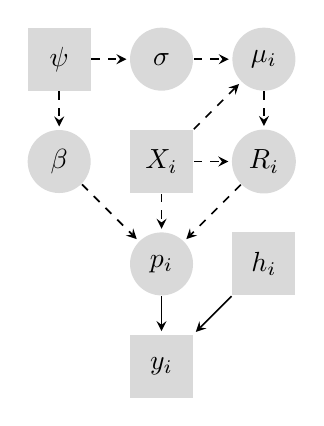
\begin{tikzpicture}[
  > = stealth,                 % arrow head style
  shorten > = 1pt,             % don't touch arrow head to node
  auto, node distance = 1.3cm, % distance between nodes
  semithick                    % thicker arrows
  ]
  
  \tikzstyle{S1}=[      % Defines style for Square 
  fill = black!15,    % Black with transparency 15%
  minimum size = 8mm  
  ]
  
  \tikzstyle{R1}=[      % Defines style for Round 
  circle,             % Changes shape
  fill = black!15,
  minimum size = 8mm
  ]
  
  % DO NOT FORGET ; AT THE END OF EACH SENTENCE!!!
  
  % Definition of the nodes
  % \node[style] (name) [relative_position] {Text};
  % Relative positions: left, right, above, below, above left, etc.
  \node[S1] (y) {$y_{i}$};
  \node[R1] (lp) [above of=y]{$p_i$};
  \node[S1] (hi) [right of=lp]{$h_i$};
  
  \node[S1] (xi) [above of=lp] {$X_i$};
  \node[R1] (bi) [left of=xi] {$\beta$};
  \node[R1] (ri) [right of=xi] {$R_i$};
  
  \node[R1] (mui) [above of=ri] {$\mu_i$};
  \node[S1] (hp) [above of=bi] {$\psi$};
  \node[R1] (sig) [above of=xi] {$\sigma$};
  
  \path[->] (lp) edge node {} (y);
  \path[->] (hi) edge node {} (y);
  \path[->,dashed] (bi) edge node {} (lp);
  \path[->,dashed] (ri) edge node {} (lp);
  \path[->,dashed] (xi) edge node {} (lp);
  \path[->,dashed] (xi) edge node {} (ri);
  \path[->,dashed] (mui) edge node {} (ri);
  \path[->,dashed] (hp) edge node {} (bi);
  \path[->,dashed] (hp) edge node {} (sig);
  \path[->,dashed] (xi) edge node {} (mui);
  \path[->,dashed] (sig) edge node {} (mui);
  \end{tikzpicture}

\end{document}

